\documentclass[conference]{IEEEtran}
\IEEEoverridecommandlockouts
\usepackage{cite}
\usepackage{amsmath,amssymb,amsfonts}
\usepackage{graphicx}
\usepackage{booktabs}
\usepackage{url}
\usepackage{placeins}
\hyphenation{XCCNet Kermany Grad-CAM}
\begin{document}
\title{Reproducing XCCNet for Pediatric Pneumonia: Focal Loss Does Not Help, and the Lung Mask Hurts}
\author{\IEEEauthorblockN{Kartik Yadav, Gangadhar Yadav, and Sahil Sarawgi}}
\maketitle

\begin{abstract}
We reproduce XCCNet for pneumonia-versus-normal classification on the Kermany pediatric chest X-rays. XCCNet uses a dilated CNN and a frozen CLIP encoder. The code is not public. We rebuild the model from the paper without the GAN and without rib suppression. Our first run on the stratified 80/10/10 split reaches 94.87\% test accuracy. The paper reports 97.18\% for that setting. Its precision and recall imply 94.84\% accuracy at our class mix.

Most errors are normal films that the model calls pneumonia. Before the code, we predicted that focal loss would raise specificity from 85\% to 88--91\%. Over three seeds, specificity fell to 79.1\%. AUC stayed at 0.975, against 0.978 for cross-entropy. With the threshold tuned on validation, both losses reach the same specificity. Focal loss only rescaled the scores.

A second ablation removes the lung mask. Accuracy rises from 92.7\% to 95.8\%, against our prediction. AUC rises from 0.978 to 0.993. Grad-CAM and the mask coverage suggest that the adult-trained mask cuts off lung tissue in child films. We make no clinical claim.
\end{abstract}
\begin{IEEEkeywords}
Pediatric pneumonia, chest X-ray, reproduction, focal loss, lung segmentation, Grad-CAM.
\end{IEEEkeywords}

\section{Introduction}
Pneumonia is a leading cause of death in children under five. A chest X-ray is the usual first test. A trained radiologist reads the film. Kermany \textit{et al.} released 5{,}856 pediatric chest X-rays from Guangzhou in 2018~\cite{kermany2018}. Many deep learning papers report pneumonia-versus-normal accuracy on this set. The reported range is 86\% to above 99\%.

These numbers are hard to compare. Papers that keep the official 624-patient test report 86\% to 95\%~\cite{kermany2018,rajaraman2018,salehi2021,ayan2021}. Papers that pool the data and use an 80/10/10 split report about 99\%~\cite{raghaw2024,choudhury2026}. Most papers report accuracy, precision, recall, and F1. Few papers report specificity or AUC. Pneumonia films outnumber normal films by about 3 to 1, so accuracy can hide errors on the normal class.

We reproduce XCCNet~\cite{raghaw2024} on the paper's split. We add specificity and AUC. Our model makes most of its errors on normal films. We test one change, focal loss~\cite{lin2017}. We stated the prediction before we wrote the code.

We compare focal loss with the baseline at a threshold tuned on validation. This comparison shows whether a gain is only a shift of the threshold. We also run one ablation with the lung mask removed.

We make three contributions. We reimplement XCCNet without its GAN and rib suppressor, and we report specificity and AUC. We check the paper's accuracy against its own precision and recall. We test a focal-loss hypothesis that we stated in advance, with a threshold control, a lung-mask ablation, and a failure analysis.

\section{Related Work}
Kermany \textit{et al.} froze an ImageNet Inception V3. They reached 92.8\% accuracy and 96.8\% AUC on the 624-patient test~\cite{kermany2018}. Rajaraman \textit{et al.} cropped the lungs with an atlas, and accuracy rose to 96.2\%~\cite{rajaraman2018}. Stephen \textit{et al.} trained a small CNN from scratch~\cite{stephen2019}. Rahman \textit{et al.} compared four ImageNet networks, and DenseNet201 gave the best result~\cite{rahman2020}. Salehi \textit{et al.} used SMOTE and warned that films from one child can occur in the train set and in the test set~\cite{salehi2021}.

Ayan \textit{et al.} and Kundu \textit{et al.} used ensembles, and the accuracy of Kundu \textit{et al.} fell from 98.81\% to 86.95\% on RSNA films~\cite{ayan2021,kundu2021}. Chauhan \textit{et al.} used class weights in a network with 388k parameters~\cite{chauhan2025}. Choudhury fine-tuned ResNet50 to 99.43\% on an 80/10/10 split~\cite{choudhury2026}. XCCNet joins a dilated CNN, CLIP~\cite{radford2021}, a contrastive term, a GAN for extra normal films, and rib suppression. XCCNet reports 99.76\%~\cite{raghaw2024}. None of these ten papers uses focal loss.

\section{Method}
\subsection{Baseline}
The spatial branch has five dilated $3\times3$ convolution blocks. The dilation is 2, and the filter count goes from 32 to 512. Each block has batch norm, ReLU, $2\times2$ pooling, and dropout 0.1. A $1\times1$ convolution maps the final $8\times8\times512$ map to 2{,}304 values.

The global branch is a frozen CLIP ViT-B/32~\cite{radford2021}. Its output has 512 values. We join the two vectors (2{,}816 values). A two-layer head with a sigmoid output reads the joined vector. The loss is Eq.~15 from the paper:
\begin{equation}
L = \phi\,L_{\text{con}} + (1-\phi)\,L_{\text{cls}} + \lambda\,L_{1},\qquad \phi = \tfrac{1}{e+1},
\end{equation}
$L_{\text{con}}$ is a symmetric InfoNCE loss between the two branches. $L_{\text{cls}}$ is binary cross-entropy. The symbol $e$ is the epoch. We resize each image to $256\times256$. We enhance each image with CLAHE (clip 2.0, $8\times8$ tiles). A lung mask from the public ChestX-Det PSPNet~\cite{cohen2022} sets pixels outside the lungs to zero.

Kermany has no masks for the ResUNet++ in the paper. A weighted sampler balances the two classes in each batch. Training uses Adam at $10^{-4}$ and a batch size of 16. On a validation plateau, the learning rate falls to $0.3$ times its value. Early stopping uses a patience of 5 epochs.

\textit{Not reproduced.} The paper gives no layer sizes and no weights for the GAN. Rib suppression needs paired bone-suppressed images. Kermany does not contain those images.

\subsection{Our change: focal loss}
We replace binary cross-entropy in $L_{\text{cls}}$ with focal loss~\cite{lin2017}:
\begin{equation}
L_{\text{focal}} = -(1-p_t)^{\gamma}\log p_t,\qquad \gamma = 2,
\end{equation}
$p_t$ is the predicted probability of the true class. A film that the model already classifies correctly at $p_t = 0.95$ keeps only $0.0025$ of its loss. No other setting changes.

\textit{Hypothesis and prediction (stated before the code).} Most errors are normal films that look a little like pneumonia. Focal loss moves the gradient toward hard films. Specificity should rise from 85\% to 88--91\%. Sensitivity should stay within 1 point, and AUC should stay within $\pm0.005$. We noted one risk. The sampler already balances the classes.

\subsection{Controls}
Row A$'$ uses the saved baseline scores. Its threshold maximises sensitivity plus specificity on the validation set (Youden's J). This row needs no new training. If focal loss beats row A$'$, then the change altered what the model learned. If focal loss does not beat row A$'$, then the change only moved the threshold. Row C removes the lung mask. We predicted a fall in accuracy of 0.5--2 points, because the model can use text markers and edges when the mask is absent.

\section{Experiments}
\textit{Data.} The films are the Kaggle mirror of Kermany~\cite{kermany2018}: 1{,}583 normal films and 4{,}273 pneumonia films. We pool the films and split them 80/10/10 per class with seed 42. The train set has 4{,}686 films. The validation set has 585 films. The test set has 585 films (427 pneumonia, 158 normal). Every run uses the same split.

\textit{Protocol.} We train each row with three seeds (42, 1, and 2). Validation accuracy selects the epoch. We evaluate the test set once per run. Pneumonia is the positive class. Sensitivity is recall on pneumonia films. Specificity is recall on normal films.

The hardware is one free Colab T4 GPU. A run takes 3--10 minutes after the image cache exists.

\begin{table}[t]
\caption{Test results, mean $\pm$ std over three seeds. FP and FN are mean counts out of 158 normal films and 427 pneumonia films.}
\label{tab:ablation}
\centering
\footnotesize
\setlength{\tabcolsep}{3pt}
\resizebox{\columnwidth}{!}{%
\begin{tabular}{@{}lccccc@{}}
\toprule
Row & Acc \% & Sens \% & Spec \% & AUC & FP / FN \\
\midrule
A: baseline & 92.71$\pm$0.55 & 95.32$\pm$1.87 & 85.65$\pm$3.25 & .978$\pm$.004 & 22.7 / 20.0 \\
A$'$: A, val threshold & 92.42$\pm$0.69 & 93.29$\pm$1.51 & 90.08$\pm$2.22 & .978$\pm$.004 & 15.7 / 28.7 \\
B: focal $\gamma{=}2$ & 91.68$\pm$0.39 & 96.33$\pm$1.08 & 79.11$\pm$2.53 & .975$\pm$.003 & 33.0 / 15.7 \\
C: no lung mask & 95.78$\pm$0.26 & 97.97$\pm$0.36 & 89.87$\pm$1.90 & .993$\pm$.001 & 16.0 / \phantom{0}8.7 \\
\bottomrule
\end{tabular}}
\end{table}

\begin{table}[t]
\caption{Prediction versus result.}
\label{tab:pred}
\centering
\footnotesize
\begin{tabular}{@{}lll@{}}
\toprule
Row & Predicted & Result \\
\midrule
A & AUC 0.97--0.99 & 0.978 (correct) \\
A$'$ & Spec $+$2--5, sens $-$1 & Spec $+$4.4, sens $-$2.0 \\
B & Spec 88--91\%, AUC $\pm$.005 & Spec 79.1\% (wrong), AUC $-$.003 \\
C & Acc $-$0.5 to $-$2 & Acc $+$3.1 (wrong) \\
\bottomrule
\end{tabular}
\end{table}

\section{Results and Discussion}
\subsection{Focal loss}
Table~\ref{tab:ablation} shows a drop in specificity of 6.5 points with focal loss. Sensitivity rose by 1.0 point. AUC did not change beyond the variation across seeds. The specificity prediction was wrong. The AUC prediction was right (Table~\ref{tab:pred}).

The scores explain this result. With cross-entropy, 78\% of test films score below 0.1 or above 0.9. With focal loss, 35\% of test films score in that range. The median normal film moves from 0.08 to 0.35. Focal loss gives easy films less weight, and the scores move toward the middle. The sampler gives the model equal counts of each class.

Pneumonia films still hold more of the remaining loss, so more normal films cross 0.5. We tune the threshold on the validation set for both models. Both models reach 90.1\% specificity. Focal loss has a slightly lower sensitivity (92.4\% against 93.3\%). Row B does not beat row A$'$. Focal loss rescaled the scores, and the rank order of the films stayed the same.

The noted risk occurred. The sampler already balanced the two classes.

\subsection{Lung mask}
When we removed the mask, every metric rose. This result disagrees with our prediction. Accuracy rose by 3.1 points. False negatives fell from 20.0 to 8.7. The spread across seeds became smaller.

Adult films at $512\times512$ supplied the training data for that mask model. We run that model on child films at $256\times256$. In seed 42 of row A, normal films in the quarter with the smallest masks have a 23.4\% error rate. The other normal films have a 14.4\% error rate. Fig.~\ref{fig:failA} shows normal films with a missing lower lobe, or with most of one lung absent. Those scores are 0.93--0.98.

Grad-CAM often marks the mask edge, the diaphragm line, and the black area below the lungs. A higher score with the mask removed does not prove a better model. With the mask removed, the model can also use the ``R'' marker, the film borders, and body size. Some row C failures have Grad-CAM marks in the lower corners (Fig.~\ref{fig:failC}). Films from one hospital cannot separate a real lung finding from such a shortcut.

\begin{figure*}[t]
\centering
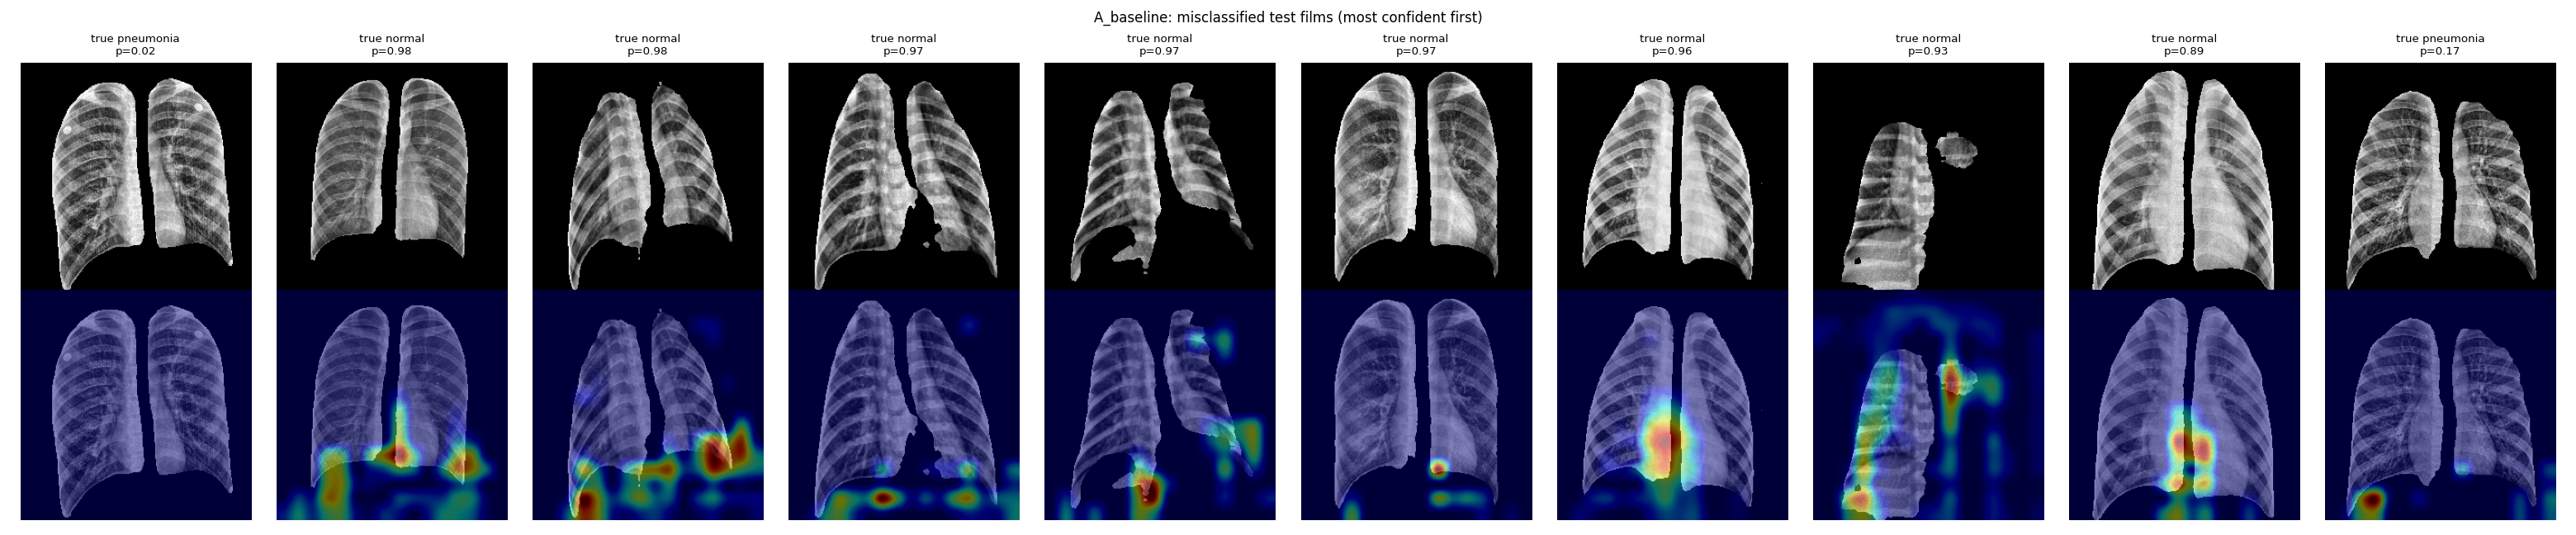
\includegraphics[width=\textwidth]{figures/failures_A.png}
\caption{Row A (baseline, seed 42): the ten test errors with the highest confidence. The top row is the input after CLAHE and the lung mask, with the true label and the predicted probability. The bottom row is Grad-CAM. On several normal films, the mask removes part of the lung.}
\label{fig:failA}
\end{figure*}

\begin{figure*}[t]
\centering
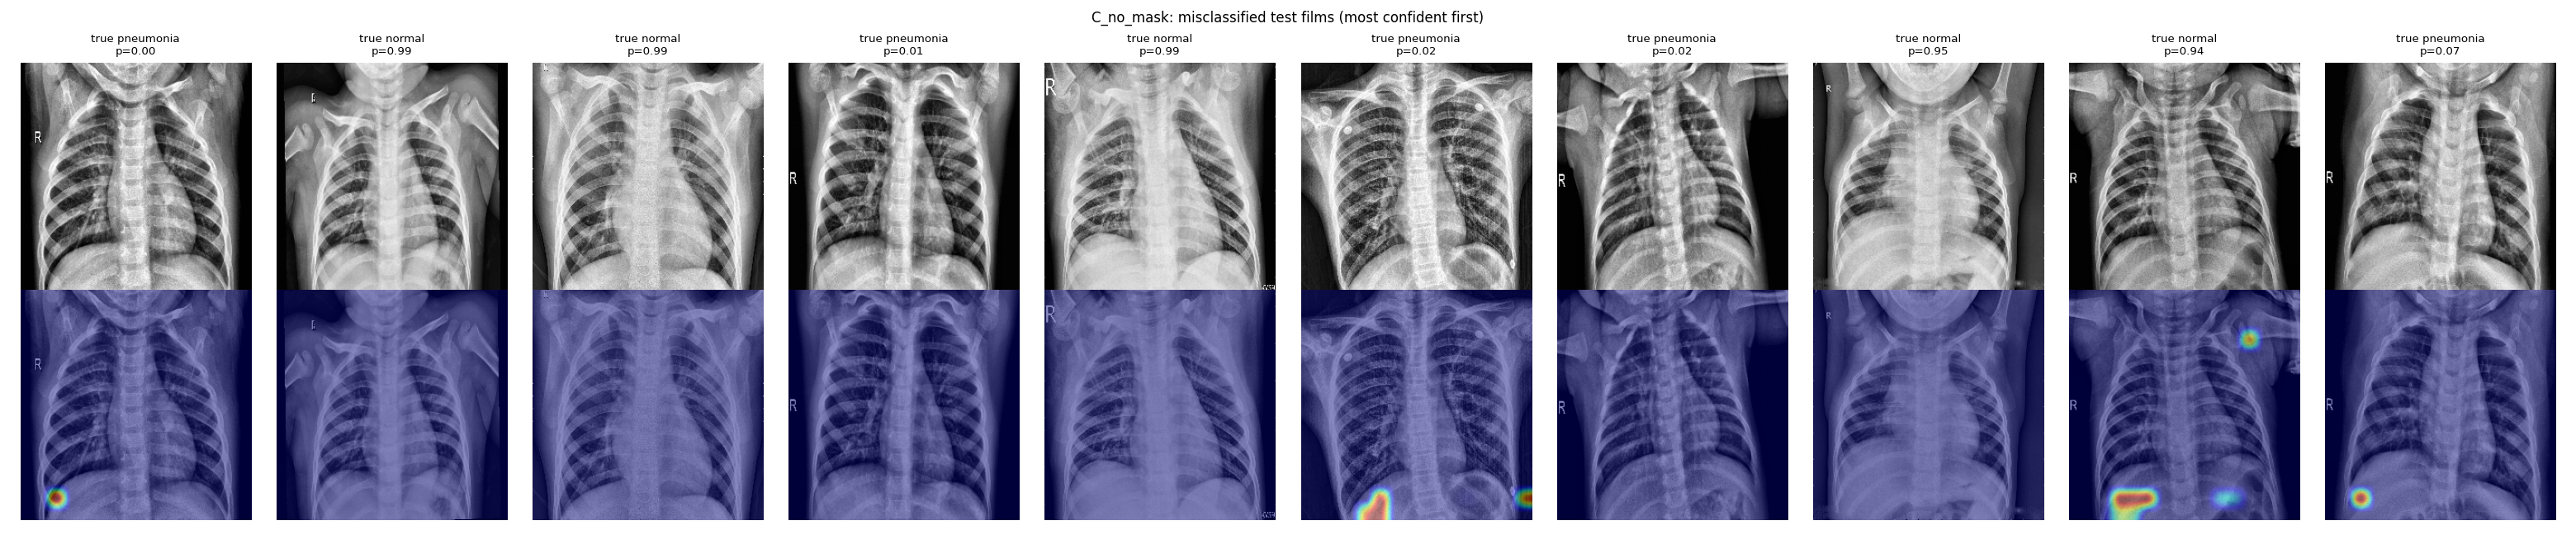
\includegraphics[width=\textwidth]{figures/failures_C.png}
\caption{Row C (no lung mask, seed 42): the ten test errors with the highest confidence. Some Grad-CAM marks lie in the lower corners, outside the lungs.}
\label{fig:failC}
\end{figure*}

\subsection{Failure analysis}
In every row, the most common error is a normal film that the model calls pneumonia (Fig.~\ref{fig:cm}). Kaggle file names label each pneumonia film as bacterial or viral. We did not train on that split. For row A, recall is 85.7\% on normal films, 96.5\% on bacterial films, and 93.4\% on viral films.

Viral pneumonia is a faint haze across both lungs. A viral film is closer to a normal film than a dense bacterial patch is. Ayan \textit{et al.} report the same weak viral class~\cite{ayan2021}.

The most confident miss in row A has $p = 0.02$. That film shows pneumonia, and the lungs look clear after CLAHE. The case may be very mild, or the label may be wrong. We cannot tell without a radiologist.

\begin{figure}[t]
\centering
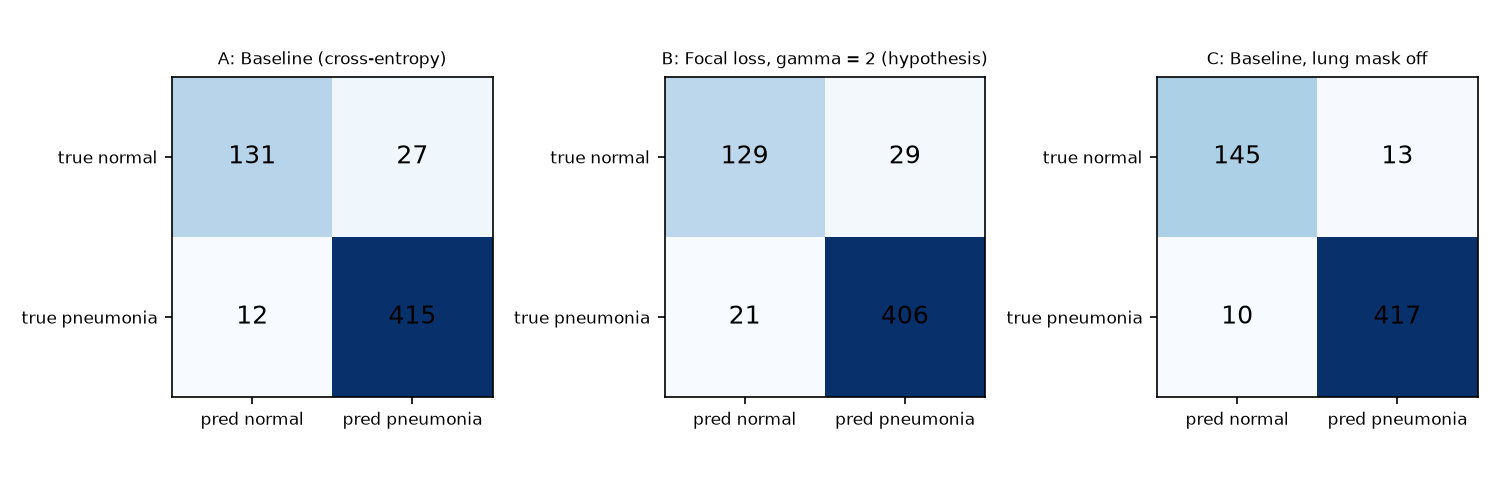
\includegraphics[width=\columnwidth]{figures/confusion_matrices.png}
\caption{Confusion matrices at a threshold of 0.5, seed 42.}
\label{fig:cm}
\end{figure}

\begin{figure}[t]
\centering
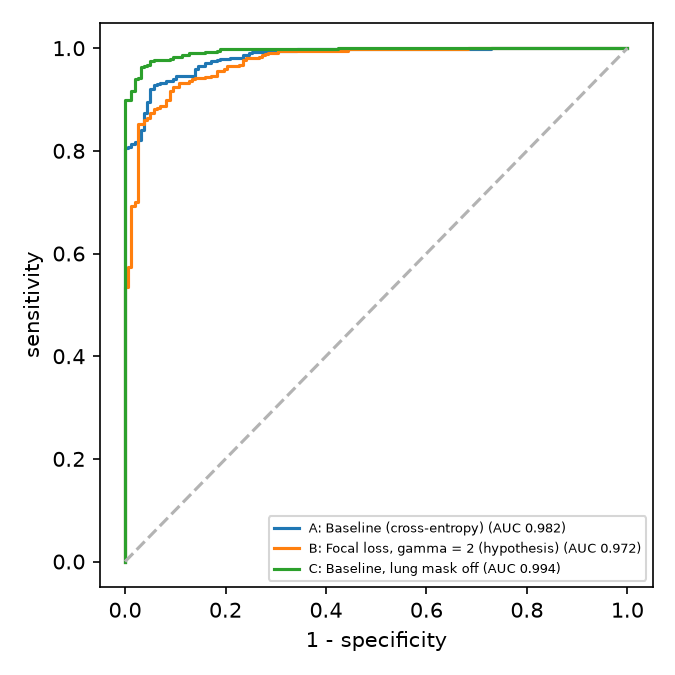
\includegraphics[width=0.8\columnwidth]{figures/roc_curves.png}
\caption{Test ROC curves, seed 42.}
\label{fig:roc}
\end{figure}

\subsection{Reproduction gap}
The paper reports 97.18\% accuracy, 94.52\% precision, and 98.65\% recall for its setting without the GAN~\cite{raghaw2024}. At our mix of 427 pneumonia films and 158 normal films, that precision and recall give 94.84\% accuracy. Our first run reached 94.87\%. The value 97.18\% fits only a test set with a different class mix. In that first run, file order depended on the disk. We could not rebuild that split.

We sorted the files before the later split. On that fixed split, the baseline averages 92.71\%. Part of the drop of about 2 points comes from which films enter the test set. Across seeds, specificity moves from 82.9\% to 89.2\%. A comparison that uses only one seed would not be reliable.

Other differences from the paper remain. Those differences are the absent GAN, the absent rib suppressor, the stand-in lung mask, and the learning rate. We use $10^{-4}$ rather than $10^{-6}$, because our CNN trains from scratch.

\section{Limitations}
All films come from one hospital. The children are 1 to 5 years old. There is no external test. We cannot say whether row C uses lung findings or shortcuts.

We use the pooled 80/10/10 split from the paper. We do not use the official 624-patient test. The split assigns films, and the split does not assign children. The 427 pneumonia test films come from 373 children, and 46 of those children have two or more films in the test set. Other films from the same child are likely in the training set as well~\cite{salehi2021}. This overlap can raise the score of every row.

We ran three seeds on one split. Early stopping on validation accuracy selected epoch 2 in several runs. A different stopping rule could change the numbers. The lung mask is a substitute for the ResUNet++ from the paper. We make no clinical claim.

\section{Conclusion}
We rebuilt XCCNet without its GAN and without its rib suppressor. Our accuracy matches the accuracy implied by the precision and recall in the paper. We stated the hypothesis before the code. The hypothesis said that focal loss would cut false positives on normal films. That hypothesis was wrong. Focal loss rescaled the scores, and AUC did not change.

A tuned threshold gave the same specificity. We then removed the adult-trained lung mask. AUC rose from 0.978 to 0.993. The rise agrees with a mask that cuts lung tissue on child films. Shortcuts outside the lungs may also explain part of the rise. The next work is a mask trained on pediatric films, the official 624-patient test, and a test on films from another hospital.

\begin{thebibliography}{00}
\bibitem{kermany2018} D.~S. Kermany, M.~Goldbaum, W.~Cai \textit{et al.}, ``Identifying medical diagnoses and treatable diseases by image-based deep learning,'' \textit{Cell}, vol.~172, no.~5, pp.~1122--1131.e2, 2018.
\bibitem{rajaraman2018} S.~Rajaraman, S.~Candemir, I.~Kim, G.~Thoma, and S.~Antani, ``Visualization and interpretation of convolutional neural network predictions in detecting pneumonia in pediatric chest radiographs,'' \textit{Appl.\ Sci.}, vol.~8, no.~10, p.~1715, 2018.
\bibitem{stephen2019} O.~Stephen, M.~Sain, U.~J. Maduh, and D.-U. Jeong, ``An efficient deep learning approach to pneumonia classification in healthcare,'' \textit{J.\ Healthc.\ Eng.}, vol.~2019, p.~4180949, 2019.
\bibitem{rahman2020} T.~Rahman, M.~E.~H. Chowdhury \textit{et al.}, ``Transfer learning with deep convolutional neural network (CNN) for pneumonia detection using chest X-ray,'' arXiv:2004.06578, 2020.
\bibitem{salehi2021} M.~Salehi, R.~Mohammadi, H.~Ghaffari, N.~Sadighi, and R.~Reiazi, ``Automated detection of pneumonia cases using deep transfer learning with paediatric chest X-ray images,'' \textit{Br.\ J.\ Radiol.}, vol.~94, p.~20201263, 2021.
\bibitem{ayan2021} E.~Ayan, B.~Karabulut, and H.~M. \"Unver, ``Diagnosis of pediatric pneumonia with ensemble of deep convolutional neural networks in chest X-ray images,'' \textit{Arab.\ J.\ Sci.\ Eng.}, vol.~47, pp.~2123--2139, 2021.
\bibitem{kundu2021} R.~Kundu, R.~Das, Z.~W. Geem, G.-T. Han, and R.~Sarkar, ``Pneumonia detection in chest X-ray images using an ensemble of deep learning models,'' \textit{PLoS One}, vol.~16, no.~9, p.~e0256630, 2021.
\bibitem{raghaw2024} C.~S. Raghaw, P.~S. Bhore, M.~Z.~U. Rehman, and N.~Kumar, ``An explainable contrastive-based dilated convolutional network with transformer for pediatric pneumonia detection,'' arXiv:2410.16143, 2024.
\bibitem{chauhan2025} N.~Chauhan, P.~K. Gupta, and F.~Doja, ``LightPneumoNet: Lightweight pneumonia classifier,'' arXiv:2510.11232, 2025.
\bibitem{choudhury2026} A.~R. Choudhury, ``Pediatric pneumonia detection from chest X-rays: A comparative study of transfer learning and custom CNNs,'' arXiv:2601.00837, 2026.
\bibitem{lin2017} T.-Y. Lin, P.~Goyal, R.~Girshick, K.~He, and P.~Doll\'ar, ``Focal loss for dense object detection,'' in \textit{Proc.\ IEEE ICCV}, 2017, pp.~2980--2988.
\bibitem{radford2021} A.~Radford, J.~W. Kim, C.~Hallacy \textit{et al.}, ``Learning transferable visual models from natural language supervision,'' in \textit{Proc.\ ICML}, 2021, pp.~8748--8763.
\bibitem{cohen2022} J.~P. Cohen, J.~D. Viviano, P.~Bertin \textit{et al.}, ``TorchXRayVision: A library of chest X-ray datasets and models,'' in \textit{Proc.\ MIDL}, 2022, pp.~231--249.
\end{thebibliography}
\end{document}
